%%%% ijcai16.tex

\typeout{IJCAI-16 Instructions for Authors}
\documentclass{article}
% The file ijcai16.sty is the style file for IJCAI-16 (same as ijcai07.sty).
\usepackage{ijcai16}

% Use the postscript times font!
\usepackage{times}

\usepackage{cleveref}
\usepackage{url}
\usepackage{amsmath}
\usepackage{amsfonts}
\usepackage{graphicx}
\usepackage{booktabs}

\setlength{\heavyrulewidth}{1.5pt}

\DeclareMathOperator*{\argmax}{argmax}
\DeclareMathOperator*{\argmin}{argmin}

\title{Hierarchical Community Detection in Complex Networks using Growing Hierarchical Self-Organizing Maps}
\author{David McDonald \\ 
University of Birmingham, \\ Birmingham, UK  \\
dxm237@cs.bham.ac.uk
\And 
Shan He \\ 
University of Birmingham, \\ Birmingham, UK  \\
s.he@cs.bham.ac.uk}
%\author{XXXXXX XXXXXX \\
%XXXXXXXXXXXXXXXX \\
%XXXXXXXXXXXXXXXX
%\And
%XXXXXX XXXXXX \\
%XXXXXXXXXXXXXXXX \\
%XXXXXXXXXXXXXXXX}

\begin{document}

\maketitle

\begin{abstract}
Detecting the community structure of complex networks is a challenging task that has occupied researchers of many disciplines for decades.
Communities often emerge of different scales and can contain within them smaller sub-communities.
%So, how can we detect the underlying hierarchical community structure of these networks? 
%Many real world problems can be modelled using a network. Analysis of these networks can provide a different perspective of the problem.
%They can also offer novel solutions that, otherwise, would not have been obvious in the original formulation of the problem.
%It is well known that networks contain an inherent community structure -- sub networks of dense connectivity -- but in complex networks, this does not fully capture all of the underlying structure of the data. Sometimes a node can belong to communities at multiple scales or hierarchies.  
%These networks often contain subsets of nodes that interact significantly more with each other than with the other nodes of the graph.
%Identifying these `communities' is imperative to understanding the interactions that comprise the complex processes modelled by the network.
%However, developing a general exploratory tool for finding the community structure of arbitrary networks is a challenging task.
%Communities often emerge at the micro and macro scale and such a tool would have to be capable of detecting this inherently hierarchical construction even when the number of communities and scales are unknown.
%Here, we propose 
%We propose using a variant of the self-organizing map that can grow an arbitrary map topology to encapsulate the community structure of any given network in such a way that the topology of the community is preserved, and that can expand any neuron into a new map for communities at different scales. 
%Here we use a variant of the self-organizing map to build maps of arbitrary shape and selectively expand areas of the search space for exploration at a finer level of granularity for this task.
We show that the so-called Growing Hierarchical Self-Organizing Map can detect the communities at multiple scales that comprise complex networks and can preserve the topological information contained within them.
% such as the positions of communities relative to other communities in the network. 
Results on small real-world benchmark networks, as well as synthetic networks, suggest that this approach can find the underlying community structure of a network, even when the mixing factor between communities is high. 
\end{abstract}

\section{Introduction}
Most real-world networks contain subsets of nodes that contain a higher degree of inter-connectivity than the rest of the network
% \cite{palla2005uncovering}. 
\cite{lancichinetti2009detecting}.
These subsets are commonly referred to as communities. 
A rigorous definition for a `community' within a network still seems to elude the scientific community \cite{lancichinetti2009detecting}.
However, the most popular definition among scholars is the planted l-partition model. 
This was popularised thanks to Girvan and Newman in their seminal work \cite{girvan2002community} and states that as long the probability of a node being connected to its group is greater than the probability of it being connected to the rest of the graph, then those groups are communities. 

`Community detection' is the name given to the problem of finding the underlying community structure in a given network \cite{girvan2002community}. 
%Many complex problems can be represented as a network and many large networks modelling real world interactions have been shown to follow the same scale-free power-law distribution \cite{barabasi1999emergence}. 
Since many complex problems can be represented as a network, community detection has proven to be useful in seemingly disconnected areas of study, such as social \cite{barber2007modularity}, biological \cite{fortunato2007resolution}, and world-wide-web \cite{danon2006effect} analysis.

Most real world networks do not solely contain communities at one scale \cite{lancichinetti2009detecting,yang2013hierarchical}. 
They contain super communities that may contain sub-communities, that may, in turn, contain their own sub communities.
And so on. 
Delving deeper into the community structure may offer some insight into how these processes work.
%For example, a network of interest in a scientific paper may contain super communities corresponding to the scientific community, hobbyists and the author's own friends and family. 
%Zooming in on the scientific community, one may notice sub-communities of various related academic disciplines such as Mathematics, Biology, and Physics. 
%Uncovering the multiple levels of community structure in the network can provide more information from the same underlying data than finding only communities at one level. 
For example, hierarchical analysis of protein-protein interaction networks may help to identify subsets of functionally-related proteins that interact together strongly within an established community representing some biological process.

%TODO gap in field
But, a general community detection algorithm does not yet exist.
Many existing algorithms suffer from a number of issues. 
To name a few:
The number and scale of communities must be known a-priori, which in most real applications, is infeasible.
Additionally, the relationships between communities, both one the same level and at different ones, is lost.
Identifying not only the community itself, but its position in the network as a whole, provides further insight into the often abstract interactions that comprise complex networks and so preserving this information when analysing a network is paramount.
And, in some cases, the algorithms cannot deal with special cases: for example, modularity-based methods suffer from the so-called `resolution limit' \cite{fortunato2007resolution}.
 
The Growing Hierarchical Self-Organizing Map (GHSOM), which was first described by Dittenbach et al. \cite{dittenbach2000growing},
% and then expanded upon in  \cite{dittenbach2002uncovering,rauber2002growing}, 
offers a unique solution to these problems .
It uses the topology-preserving property of self-organizing maps, in conjunction with the ability for maps to grow into arbitrary shape completely autonomously. 
GHSOM is capable of detecting the community structure of complex networks and adapt the shape of its maps to fit the structure of the data.  
And, by selecting promising areas of the input space to expand and produce maps of finer granularity, GHSOM is capable of studying interesting areas of  the input space in greater detail.
%These properties suggest that GHSOM might be a suitable choice for a general tool for detecting communities in biological networks that so commonly feature a hierarchical structure. 
%Preserving the topology of the input space will produce a map of communities that shows the how the communities link together and super and sub community relationships in the network.
These properties suggest that GHSOM is a suitable candidate for a hierarchical community detection algorithm, and this study will explore the usefulness of GHSOM for this task.

\section{Related Work}
Over the years, numerous and varied approaches have arisen to tackle the problem of community detection. 
Readers interested in thorough reviews and in-depth algorithm comparisions are directed to  \cite{fortunato2010community}.

\subsection{Cut-Based and Spectral Approaches}
Most early work on community detection focused on `cutting' the network into modules, in such a way that the number of edges cut was minimized. 
In theory, this resulted in the best partition of the network into communities \cite{kernighan1970efficient}.
%However, this often favoured cuts of small, peripheral subgraphs, so it was adapted into ratio cut \cite{wei1991ratio}, normalised cut \cite{shi2000normalized} and min-max cut \cite{ding2001min} that took the number of nodes in each resulting sub-graph into account, and thus resulted in a partition that was more balanced.
However, this often favoured cuts of small, peripheral subgraphs, so it was adapted into ratio cut, normalized cut and min-max cut that took the number of nodes in each resulting sub-graph into account, and thus resulted in a partition that was more balanced.
Summaries of these cuts can be found in \cite{fortunato2010community}.
%\begin{align}
%Rcut(A_1,...,A_k) = \sum_{i=1}^K \frac{cut(A_i,\bar{A_i})}{|A_i|}
%\end{align}

%More recently, `conductance' has become a common term for defining a good cut. 
%Conductance, defined as:
%\begin{align}
%\phi(S) = \frac{c_s}{\min(Vol(S),Vol(V \setminus S)} 
%\end{align}
%with
%\begin{align}
%c_s = |\{(u,v) : u \in S, v \not\in S\}|
%\end{align}
%is concerned with edges, rather than vertices, and has been used to detect communities in bipartite networks \cite{barber2007modularity} and combined with PageRank \cite{andersen2006local}. 

Spectral clustering dates back to the work of Donath and Hoffman in 1973 \cite{donath1973lower}. 
However, it was popularized in the early 2000s \cite{ng2002spectral}. 
%However, it was popularized by the works of Shi and Malik \cite{shi2000normalized}, Ng et al. \cite{}, and Ding \cite{ding2004tutorial}.
Spectral methods rely upon constructing `Laplacian' matrices from the raw network data and eigen-decomposing them. 
Clustering the resulting eigenvectors results in clusters of the original data points. 
Spectral approaches have many advantages over other techniques and, as a result, they have become popular in the machine learning community for clustering  on non-linear manifolds. 
%According to \cite{von2007tutorial}, `these methods do not make assumptions about the form of the clusters' and are capable of correctly identifying typically challenging clusters, such as the famous two spirals example. 
%For community detection, they have the additional benefit of efficiency, especially if the graph adjacency matrix is sparse. 
%They are also able to detect which nodes form connected components within a general network where nodes are not always connected \cite{von2007tutorial}. 
Spectral methods can also be combined with traditional hierarchical modularity methods \cite{donetti2004detecting}.
% where the graph was eigen-decomposed and projected into a $g$-dimensional subspace and then the resulting points were clustered to maximize modularity.

%\subsection{Evolutionary Approaches}
%Approaches using evolutionary algorithms typically encode the community structure of a graph using the locus based adjacency first proposed in \cite{park1998genetic}. The genotype consists of $N$ genes and $j$ appearing in gene position $i$ is interpreted as nodes $i$ and $j$ belonging to the same community. This representation was used to great effect as part of the MOCK algorithm \cite{handl2007evolutionary} which solved the community (or in this case, clustering) problem using a multi-objective optimisation algorithm that attempted to balance compactness and connection of the clusters, and used several novel genetic operators. Variation modifiers are used in \cite{pizzuti2008ga} to reduce the search pace by taking into account the correlations of the nodes.



%Further early work includes the Metis algorithm \cite{karypis1998fast}, that finds the best split of a graph into two equal sized pieces, and the MQI algorithm \cite{gallo1989fast}. 
Further work includes the Markov Clustering algorithm (MCL) that simulates a diffusion process on a graph by repeatedly performing stages of expansion and inflation and only keeping the $k$ largest elements for efficiency \cite{van2001graph}. 
%His algorithm has since found use in Miru, a commercial 3D network visualization software, to cluster very large graphs quickly.

\subsection{Modularity-Based Approaches}
The seminal work of Girvan and Newman \cite{girvan2002community} marked a significant advance in the field by providing the first quantitative measure of a community: modularity. 
The modularity of a partition of a network 
%defined as
%\begin{align} 
%\label{modularity}
%Q = \sum_{s=1}^m \bigg[ \frac{l_s}{L} - \bigg( \frac{d_s}{2L} \bigg)^2\bigg]
%\end{align}
scores a network partition by comparing the number of links inside a given module with the expected number that would be found in a random graph of the same size and degree sequence. 
%Here, $m$ is the number of modules in the partition, $l_s$ is the number of links in module $s$, $L$ is the total number of links in the network and $d_s$ is the total degree of the nodes in $s$. 
%The first term in equation \ref{modularity} is the fraction of links inside $s$ and the second term represents the expected fraction of random links in the graphs to be in the module. 
Girvan and Newman propose a hierarchical divisive algorithm that removes edges based on their `betweenness' (the number of shortest paths from two nodes in the network that go through them) until the modularity quality function is maximized. 
The early work of Girvan and Newman has since been expanded upon.
For example, edge clustering in favour of edge-betweenness \cite{radicchi2004defining}, iteratively adding links to a module based on their expected increase in modularity \cite{clauset2004finding}, and multi-stage local optimization \cite{blondel2008fast}.

%Radicchi at al. \cite{radicchi2004defining} used a similar divisive algorithm, but instead of edge betweenness, used an edge clustering co-efficient based on loops in the network. 
%They also proffers the notion of `strong' and `weak' communities based on their internal and external degrees. 
%Clauset et al. \cite{clauset2004finding} sped up Newman's the agglomerate algorithm in \cite{newman2005power} to iteratively add links to a module based on their expected increase in modularity. 
%A similar approach was performed by Guimera and Amaral \cite{guimera2005functional} with simulated annealing. 
%Blondel et al. \cite{blondel2008fast} offered a multi-stage local optimization of Girvan and Newman's algorithm that iteratively replaced communities with a single node. 

%Other work with modularity-based quality scores include the work of Rosvall and Bergstrom \cite{rosvall2007information} that translated the problem of community detection into the problem of optimally compressing the information in a graph such that the most information can be uncovered when the compression is decoded. 
%They used simulated annealing to minimize a function that represented both compression and data loss. 
%While slow and computationally expensive, this approach was also shown to work well with dynamic processes in his later work \cite{rosvall2008maps}. 

%It has been shown that modularity-based approaches have their limitations. 
%In particular, Fortunato and Bartelemy \cite{fortunato2007resolution} show what they referred to as the `resolution limit' - that modularity-based approaches can fail to identify communities that are smaller in size than a scale that depends on the size of the network, and this results in incorrect community division in the cases when even small communities must be considered. 
%But it has been shown that resolution limit can be overcome.
%Ronhovde and Nussinov \cite{ronhovde2010local} does not compare to a null model as in equation \ref{modularity}, but instead penalize communities for any missing edges. 
%This provided good results even on very small communities compared to the size of the overall network. 

\subsection{Statistical Approaches}
Statistical approaches have been shown to deduce the best model to fit the data represented in the graph structure, which may not necessarily be communities \cite{newman2004finding}.
They have also been used to show the trade off between using heuristics to reduce the search space and optimization of a constrained quadratic function \cite{yang2013hierarchical}.
%In \cite{newman2004finding}, Newman and Girvan used Bayesian inference to deduce the best model to fit the data represented in the graph structure.
%His algorithm was capable of finding the best group structure for any graph, no just a community structure, but required the number of groups to be know a-priori. 
%Probability theory was also used by Yang et al. in \cite{yang2013hierarchical} for the construction of their Probabilistically Mining Communities (PMC) algorithm. 
%PMC offers a trade off between using a random walk as a heuristic to reduce the search space and optimizing using a constrained quadratic optimization function. 
%Furthermore, `label propagation' methods proposed by Raghavan in \cite{raghavan2007near} have had success at detecting communities in real time \cite{leung2009towards}.


\subsection{Neural Network Approaches}
The deep learning community has began to explore the possibilities of using neural networks for clustering in the graph domain. Convolutional neural networks (CNNs), powerful machine learning tools that have proven very successful for challenging classification tasks that have recently been generalised to take a graph input \cite{defferrard2016convolutional}. 
CNNs have also been used for semi-supervised learning on graphs, where the they are capable of learning both graph structure and node features \cite{kipf2016semi}. 
%Here, some nodes are labelled the labels of every other node are inferred by the model, which is capable of learning both the graph structure and node features.  

\section{Hierarchical Community Detection}
%In many practical networks, partitioning a network into a cover does not accurately reflect the inherent community structure of the data. Sometimes, nodes can belong to more than one community -- sometimes communities overlap. The first algorithm to consider overlapping communities was CFinder in 2006 \cite{adamcsek2006cfinder}. Drawing from the earlier work of Palla et al. and the Clique Percolation Method (CPM) \cite{palla2005uncovering}, CFinder considered communities as the unions of k-cliques and so rolled k-cliques across the graph to detect communities. While computationally expensive, it was able to deal with overlapping cases, and opened the door for further study. Shen et al. proposed EAGLE in 2009 \cite{shen2009detect} that used maximal cliques, an agglomerative hierarchical structure and a modified modularity quality function that detected complex overlapping community structures.

The hierarchical nature of modularity-based clustering methods can allow them to detect communities at different scales. 
\cite{lancichinetti2009detecting} used local optimization to maximize a fitness function with a parameter that controlled the size of communities detected.
Other work includes multi-scale quality functions that can uncover hierarchical communities and produce several different partitions of a graph, the post-processing of clusters found by hierarchical methods (encoded in a dendogram) \cite{pons2011post}, and Bayesian non-negative matrix factorisation that performs `soft-partitioning' and assigns node participation scores to modules \cite{psorakis2011overlapping}.


%Complex networks very often contain communities at different scales -- communities within communities -- and it is informative to investigate the communities identified at different levels of hierarchical algorithms to uncover these. 
%The first algorithm to look for both overlapping and hierarchical communities was proposed by Lancincetti et al. \cite{lancichinetti2009detecting}, where they aim to locally maximize a fitness function based on the fraction of connections going in and out of a subset of nodes, and a parameter $\alpha$ that controlled the scale of the communities uncovered.
%\begin{align}
%f_G = \frac{k_{in}^G}{(k_{in}^G + k_{out}^G)^\alpha}
%\end{align}
%where $k_{in}^G$, and $k_{out}^G$ are the total internal and external degree of the nodes going into community $G$, and $\alpha$ controls the size of communities. 

%Potts methods have also shown good tolerance towards communities that overlap. 
%Both \cite{reichardt2006statistical} and \cite{ronhovde2009multiresolution} look for the ground state of spin and interpret the spin configuration that minimizes energy of spin glass as the underlying community structure of the state. 
%Due to user-controlled resolution parameters, they are able to identify overlapping and hierarchical communities.



\section{Self-Organizing Maps}
Also known as the Kohonen Map after its creator Teuvo Kohonen, the Self-Organising Map (or SOM) is a topology-preserving neural network that performs unsupervised learning of a input space onto a low-dimensional discrete map \cite{kohonen1990self}. 
Unlike other neural networks, SOM uses competitive learning - determining the `winning' neuron by some distance function -- called Learning Vector Quantization (LVQ), rather than a supervised training approach. 
Weights of all neurons are adjusted proportional to their distance to the winning neuron. After many epochs of organization in this way, the resulting map perseveres the topology of the input space, meaning that features that appear together in the input space will appear together in the map.


\subsection{SOM in the Literature}
%SOM for classification has been throughly researched \cite{kiang2001extending} thanks to Learning Vector Quantization (LVQ), an extension to SOM that divides the input space into `Voronoi Regions' based on Euclidean distance to the weight vector of each neuron, proposed by Kohonen humself \cite{kohonen1995learning}. 
%This allows inputs to be classified based on which Voronoi Region it falls in. 
%In the past, SOM has had successes with medical diagnosis \cite{vercauteren1990classification}, image and character recognition \cite{sabourin1993modeling,delbimbo1993three}, and speech recognition \cite{leinonen1993self}. 


Explicit community detection on graphs using SOM remains largely under-researched. 
But, by constraining neuron weights to move along edges in the graph, SOM has shown promise for use on raw graphs, at least for the simple case of the travelling salesman problem \cite{yamakawa2006self}.
SOM has been shown to perform an implicit form of multi-dimensional scaling (MDS) for graph embedding and visualization in the two and three dimensional plane \cite{bonabeau2002graph}.
%Yamakawa et al. \cite{yamakawa2006self} implemented a SOM variation that could take a graph as an input and output a two-dimensional topology-preserving lattice that represented a solution to the travelling salesman problem. 
%They constrain the weights of the neurons in the network to only point to edges on the graph and
%They represent neuron weights as
%\begin{align}
%\textbf{w} = (n_i, n_j, \beta)
%\end{align}
%where $n_i$ is a node on the graph, $n_j$ is a neighbour of $n_i$, and $\beta\in[0,1]$ represents how far along the edge connecting $n_i$ and $n_j$ the weight vector is pointing. 
%weights are pulled along the shortest path on the graph from their current position to the input vector.

%Clustering with SOM, remains relatively under researched.
%Fritzke \cite{fritzke1994growing} offers both an unsupervised and supervised SOM algorithm for clustering. 
%Additionally, his algorithm automatically found the best network structure and size using controlled map growth and neuron removal.
%Both \cite{kiang2001extending} and \cite{vesanto2000clustering} cluster the output of SOM using k-means and this is shown to outperform the clustering achieved by k-means and hierarchical methods alone.



%Self-organizing maps have also been as an implicit form of Multi-Dimensional Scaling (MDS) for graph embedding and visualization on a two and three dimensional plane \cite{bonabeau2002graph}. Bonabeau cited the seminal work of Kernighan and Lin \cite{kernighan1970efficient} who identified that MDS can allow for clusters and communities within a graph to be more easily identifiable even before a cover is found. The embedding found by SOM satisfied the requirement of MDS to preserve the relative relationships of vertices in the graph, and this allowed the vertices to be easily clustered into communities in $\mathbb{R}^2$. He found particularly good results on large networks, where SOM was able to more easily learn the distribution of training vectors but admits that more work could be at making the connection between MDS and SOM more rigorous.

For clustering in general with SOM, unsupervised and supervised algorithms have been proposed that control map growth and neuron removal \cite{fritzke1994growing}.
Additionally, clustering the output of SOM with k-means has been shown to outperform k-means and hierarchical methods alone \cite{kiang2001extending}.

\section{Method}
%The next section will outline a variation of the self-organizing map, called the Growing Hierarchical Self-Organizing Map, that does not require the number of neurons a priori and is capable of investigating areas of the input space with greater granularity if required, producing multiple maps of the same space. 
%While not a new algorithm, the novelty comes from its application in the domain of hierarchical community detection in complex networks.
The entire algorithm presented in this work consists of two main phases: projection and map construction. Projection is concerned with embedding the vertices of the network into $k$-dimensional Euclidean space. GHSOM is then used to construct two-dimensional maps of the community structure of the network at different hierarchies.
%Adapting GHSOM for community detection first requires the vertices of the network to be projected onto a Euclidean space, before hyper parameters are selected and the GHSOM is run. 

%\begin{figure}
%\centering
%\includegraphics[scale=0.4]{overall_algorithm.png}
%\caption{A flowchart providing an overview of the entire algorithm.}
%\end{figure}

\subsection{MDS Projection of Vertices}
%Let us suppose a connected network $\textbf{G}$. 
%The first step of the algorithm is to project $\textbf{G}$ into a Euclidean space, that is suitable for SOM. 
%For this, we use Multi-Dimensional Scaling (MDS). 
Multi-Dimensional Scaling was used to first project the vertices of a given network $\textbf{G}$ onto a Euclidean plane $\textbf{X}\subset\mathbb{R}^k$.
Explicit MDS was used in favour of running GHSOM on the raw network as MDS embeds based on a similarity  measure than can be changed. The embedding for one measure -- day shortest path distance -- may result in different communities than for another measure -- say sum of node degree along shortest path. And, the communities that are preserved across multiple measures may be important to the network as a whole. %TODO
 
MDS takes as input a matrix $\textbf{D}$ of distances or dissimilarities and attempts to find an embedding of each point such that the relative distances are preserved. 
Here, we use the shortest path between two nodes as the metric, as in \cite{yamakawa2006self}. 
This distance is well defined and finite for all pairs of nodes in the network since $\textbf{G}$ is a connected graph. 

%After obtaining a distance matrix $\textbf{D}$, a kernel matrix $\textbf{K}$ can be computed using double centring as follows:
%\begin{align}
%\textbf{K} = -\frac{1}{2} \textbf{C}_n \textbf{D} \textbf{C}_n
%\end{align} 
%where $\textbf{C}_n$ is the centring matrix, given by
%\begin{align}
%\textbf{C}_n = \textbf{I}_n - \frac{1}{n} \textbf{1} \textbf{1}^T
%\end{align}
%$\textbf{K}$ is eigen-decomposed and factored into
%\begin{align}
%\textbf{K} = \textbf{U} \Lambda \textbf{U}^{-1}
%\end{align}
%Since Euclidean spaces have the property that
%\begin{align}
%\textbf{K} = \textbf{X} \textbf{X}^T
%\end{align}
%then we have that the embedding matrix $\textbf{X}$ is given by
%\begin{align}
%\textbf{X} = \textbf{U} \Lambda^{\frac{1}{2}}
%\end{align}


%MDS is used as a form of dimensionality reduction: a pre-determined dimension $k$ (usually 2 or 3 for data visualization tasks) is given to the algorithm and then only the $k$ eigenvectors and eigenvalues are used to compute $\textbf{X}$ that minimize strain, given by
%\begin{align}
%strain_{\textbf{D}} (x_1, x_2, ..., x_n) = \Bigg ( \frac{\Sigma_{i,j}(k_{i,j} - \langle x_i,x_j \rangle)^2}{\Sigma_{i,j}k^2_{i,j}} \Bigg ) ^ {\frac{1}{2}} 
%\end{align}

We then use double centring to construct a kernel matrix $\textbf{K}$ from $\textbf{D}$ and eigen-decompose it. 
In order to prevent the need to specify the dimensionality of the data, $k$, a-priori, we determine $k$ dynamically as follows:
%by ordering the eigenvalues into descending order and calculating their sum. 
%$k$ was initialized to $k=n$ and then the sum of the first $k$ eigenvalues was computed and then divided by the sum of all the eigenvalues. 
%If this was greater than 0.95, then $k$ was decremented by 1 and this process was repeated. 
%With this, we are looking for the largest $k$ such that
\begin{align}
k = \argmax_k \Bigg(\frac{\Sigma_{i=1}^k \lambda_i}{\Sigma_{j=1}^n \lambda_j} \geq 0.95 \Bigg)
\end{align}
%holds. 
This ensures that 95\% of variation is preserved, no matter how many nodes in $\textbf{G}$ there are. 
Then the $k$ largest eigenvalues and their associated eigenvectors are used to compute $\textbf{X}$, giving an $n\times k$ matrix where the $i$th row gives the co-ordinates of node $i$ in $k$-dimensional space.

\subsection{The Growing Hierarchical Self-Organizing Map}
Embedding the $n$ nodes into $k$ dimensional space translates the problem of finding communities in a graph to identifying clusters in the Euclidean Space $\textbf{X}$. Since the distance (by whatever metric used) between two nodes within the same community should be smaller than two nodes belonging to two different communities, then all of the nodes within a community should be embedded closely together in $\textbf{X}$.
%And so, identifying clusters of data points in $\textbf{X}$ is the same as identifying communities in the original graph $\textbf{G}$.
For clustering in $\textbf{X}$, we use GHSOM.

\subsection{Hyper-Parameters}
GHSOM takes two additional hyper parameters to SOM. 
The first is $\epsilon_{sg}$ and this determines the size of the maps that will be created. 
The second, $\epsilon_{en}$, determines the granularity of the maps produced, or when the network should grow a new layer. 
Both of these will be discussed in more detail later in this paper.
Additionally, GHSOM uses a measure of error, that its creators, Dittenbach et al. called Mean Quantization Error (or MQE). 
Following their example, let the MQE of a single neuron $i$ be denoted $\textbf{mqe}_i$ and the MQE of an entire map $m$ be denoted $\textbf{MQE}_m$.

\subsection{$\textbf{MQE}_0$}
GHSOM begins with layer 0 comprising a single neuron map. 
This neuron is given a weight vector $\textbf{w}$ that points to the centre (the mean) of all the data points:
\begin{align}
\textbf{w} = \frac{1}{n} \sum_{i=1}^n \textbf{x}_i
\end{align}
The MQE of this neuron (and therefore this first map) is the variance of the data set:
\begin{align}
\textbf{MQE}_0 = \textbf{mqe}_0 = \frac{1}{n} \sum_{i=1}^n ||\textbf{w} - \textbf{x}_i||
\end{align} 
This is used as a benchmark for all the following layers to beat.

\subsection{Training the First Layer}
GHSOM then begins by training the first layer map. 
The first layer is initialized to just one neuron. 
The weights of this neuron is initially set to be a random vector in $\mathbb{R}^k$. 
The map is then trained as in the standard SOM algorithm, found in \cite{kohonen1990self} for $\lambda=10000$ epochs.

One training epoch consists of presenting each training pattern (the embedded nodes of $\textbf{G}$) to the map. 
For each pattern $\textbf{x}$, the `winning' neuron $i^*$ is determined as:
\begin{align}
i^* = \argmin_i  ||\textbf{x} - \textbf{w}_i||
\end{align}

The weights of every neuron in the map are then adjusted to move a little closer to $\textbf{x}$, based on how close to $i^*$ they are in the map.
\begin{align}
\textbf{w}_i(t+1) = \textbf{w}_i(t) + \eta(t) h(i, i^*, \sigma(t)) (\textbf{v} - \textbf{w}_i)
\end{align}
The weights are adjusted proportionally to the learning rate $\eta(t)$, and the neighbourhood function $h(i, i^*, \sigma(t))$, given by
\begin{align}
h(i, i^*, \sigma(t)) = \exp\Bigg(-\frac{||\textbf{r}_i-\textbf{r}_{i^*}||^2}{2\sigma(t)^2}\Bigg)
\end{align}
where $\textbf{r}_i$ is the position of neuron $i$ in the map.
The neighbourhood function preserves the topological ordering of the map, as neurons closer to the winning neuron in the map move towards $\textbf{x}$ more.
At the end of each training epoch, the order of the training patterns is shuffled. Then the neighbourhood width $\sigma(t)$ is adjusted in the following manner:
\begin{align}
\sigma(t) = \sigma_0 \exp \Bigg(-\frac{2 \sigma_0 t}{\lambda}\Bigg)
\end{align}

%Both $\eta(t)$ and $\sigma(t)$ vary with time and decrease as the number of training epochs increases. 
%This allows the movements of the weights to gradually decrease and become fine-tuned.



\subsection{Growing the Map}
After $\lambda=10000$ training epochs have passed, every node in $\textbf{G}$ is assigned to the neuron in the map whose weight vector $\textbf{w}$ points closest to it in $\mathbb{R}^k$. 
Then the $\textbf{mqe}_i$ for each neuron is calculated, as well as the overall $\textbf{MQE}_1$ of the map. 
If 
\begin{align}
\textbf{MQE}_1 \geq \epsilon_{sg} \textbf{mqe}_0
\end{align}
then the network is expanded, by inserting a single new neuron into the map, else expansion terminates.

Network expansion largely follows the example of Bernd Fritzke in \cite{fritzke1994growing} and aims to preserve a simplicial structure within the map whenever a new neuron is inserted. 
This ensures that neurons do not have too many neighbours. 
Firstly, one must identify the `error unit' $e$ -- the neuron with the greatest error in the map. 
Then retrieve the list of all of the adjacent neurons (the neighbours) of $e$ in the map.

%\subsubsection{Single Neuron in Network}
%In the case that $e$ has no neighbours (the map consists of one neuron) then a new neuron is added to the map with a random weight vector and connected to the $e$. 
%
%\subsubsection{Two Neurons in Network}
%In the case of one neighbour, the weight vector of the new neuron is given the mean of the weight vectors of the the existing two neurons in the network and then connected to both neurons. 

%\subsubsection{Greater than Two Neurons}
In the general case, the `furthest neighbour', $n_1$, of $e$ is identified. 
This is the neighbour whose weight vector points furthest away from the weight vector of $e$ in the input space. 
The furthest neighbour is then determined from the list of mutual neighbours of $n_1$ and $e$, called $n_2$. 
Next, the connection between $n_1$ and $n_2$ is broken and a new neuron is inserted with a weight vector equal to the mean of the weight vectors of $e$, $n_1$, and $n_2$. 
Finally, the new neuron is connected to every neuron that is connected to both $n_1$ and $n_2$ (including $e$ itself).
When there are $e$ has no neighbours in the map, then a new neuron is connected to $e$ with a random weight vector.
If $e$ has one neighbour, then the new neuron is connected to both neurons in the map and given a weight equal to the mean of their weights.

\subsection{Termination of Map Growth}
The map is again trained for $\lambda=10000$ epochs and $\textbf{MQE}_1$ is recalculated. If
\begin{align}
\textbf{MQE}_1 < \epsilon_{sg} \textbf{mqe}_0
\end{align}
then map growth terminates. 
Otherwise, another neuron is inserted and the training and growth process repeats.

\subsection{Adding a New Layer to the Map}
After growth for the current map has terminated, GHSOM determines whether or not to build another layer by expanding specific neurons in this one. 
Whether or not to expand is determined by $\epsilon_{en}$. 
GHSOM scans across all the neurons $i$ in the map and checks for
\begin{align}
\textbf{mqe}_i \geq \epsilon_{en} \textbf{mqe}_0
\end{align}

If a neuron $i^*$ is located with this property then a new map is constructed (again starting from one neuron). 
This time, only the subset of nodes in $\textbf{G}$ that were assigned to $i^*$ are passed to the new map. 
Training growth and expansion of new map follows exactly the same procedure as for the current map.

\subsection{Termination of GHSOM}
GHSOM continues to train, grow and expand maps until 
\begin{align}
\textbf{MQE}_m < \epsilon_{sg} \textbf{MQE}_0
\end{align}
for all maps $m$ and
\begin{align}
\textbf{mqe}_i < \epsilon_{en} \textbf{MQE}_0
\end{align}
for all neurons $i$. 
The output is then a set of maps where each neuron represents a community in $\textbf{G}$.
Neurons that were expanded contain pointers to the map that was grown from their nodes.

\section{Results}


\begin{table}
\begin{tabular}{c p{6.5cm}}
\toprule
\textbf{Network} & \textbf{Description} \\
\bottomrule
Karate & Social network of karate club \cite{zachary1977information}.\\
Dolphin & Social network of dolphins living in New Zealand \cite{lusseau2003bottlenose}.\\
Polbooks & Network of books sold by \url{www.amazon.com} and published around the 2004 presidential election \cite{girvan2002community}.\\
Football & A network of college football games in Fall 2000 \cite{girvan2002community}.\\
\bottomrule
\end{tabular}
\caption{Description of four real-world networks.}
\end{table}


\begin{table}
\centering
\begin{tabular}{ l p{2.5cm} l l }
\toprule
\textbf{Parameter} & \textbf{Description} & \multicolumn{2}{c}{\textbf{Network Type}} \\
{} & {} & Real-World & Synthetic \\ 
\bottomrule
$\eta$ & Learning rate & 0.0001 & 0.0001 \\ 
$w$ & Weight range & 0.0001 & 0.0001 \\
$\sigma$ & Neighbourhood size & 1 & 1 \\
$\epsilon_{sg}$ & Stop map growth & 0.8 & 0.8 \\
$\epsilon_{en}$ & Grow new map & 0.8 & 0.8 \\
\bottomrule
\end{tabular}
\caption{Parameter setting for both types of network.}
\label{parametersettings}
\end{table}

%\begin{table}
%\centering
%\begin{tabular}{p{1.95cm} l l l l}
%\toprule
%\textbf{Parameter} & \multicolumn{4}{c}{\textbf{Network}} \\
%{} & Karate & Dolphin & Polbook & Football \\
%\bottomrule
%\textbf{\#jobs} & 28 & 521 & 562 & 181 \\
%\bottomrule
%%$\eta$ & 0.00010 & 0.879141 & 0.999305 & 0.058690 \\
%%$w$ & 0.943492 & 0.0001 & 0.352897 & 0.066269 \\
%%$\sigma$ & 0.816632 & 0.001 & 0.649818 & 1.000 \\
%%$\epsilon_{sg}$ & 0.988303 & 0.557975 & 0.999970 &  0.450884 \\
%%$\epsilon_{en}$ & 1.000000 & 0.3 & 0.392926 & 0.300000 \\
%$\eta$ & 0.0001 & 0.879 & 0.999 & 0.0587 \\
%$w$ & 0.943 & 0.0001 & 0.353 & 0.0663 \\
%$\sigma$ & 0.817 & 0.001 & 0.650 & 1.0 \\
%$\epsilon_{sg}$ & 0.988 & 0.558 & 1.0 &  0.451 \\
%$\epsilon_{en}$ & 1.0 & 0.3 & 0.393 & 0.3 \\
%\bottomrule
%\textbf{\#comms} & 2 & 4 & 3 & 12 \\
%\textbf{\#comms det.} & 2 & 4 & 2 & 11 \\
%\textbf{NMI score} & 1.0 & 0.640 & 0.688 & 0.874 \\
%\bottomrule
%\end{tabular}
%\caption{Spearmint optimized parameter settings and NMI scores for real world networks (to 3 s.f.).}
%\label{bayes}
%\end{table}

Results were obtained using two sets of parameters for GHSOM, one for the real-world networks and one for the synthetic ones. Parameters were kept consistent across all networks to allow for fair comparison, but individual optimization of these parameters produced better results. \Cref{parametersettings} details the consistent parameter settings used for each network type.

Four representative algorithms from the literature are used for comparison: MCL \cite{van2001graph}, FM \cite{clauset2004finding}, FUC \cite{blondel2008fast}, and PMC \cite{yang2013hierarchical}.



%\subsection{Real-World Benchmarks}
%The following real world benchmark networks were used.
%
%\subsubsection{Karate}
%A social network detailing the friendships of 34 members of a university karate club in 1970s. Compiled by Zachary \cite{zachary1977information}, nodes belong to one of two communities corresponding to the split in the club between the club instructor and administrator.
%\subsubsection{Dolphin}
%A social network of the interactions of 62 dolphins living off Doubtful Sound in New Zealand. The network was first described by Lusseau in 2003 \cite{lusseau2003bottlenose}. Dolphins are divided into 4 communities based on the modularity algorithm of Girvan and Newman.
%\subsubsection{Polbooks}
%A network of books sold by \url{www.amazon.com} and published around the 2004 presidential election. Each book is connected with they were co-purchased by the same customer and are labelled by party affiliation \cite{girvan2002community}. 
%%The network is unpublished but compiled by Krebs \cite{polbooks}.
%\subsubsection{Football}
%A network of college football games in Fall 2000 \cite{girvan2002community}.


\begin{table}
\centering
\begin{tabular}{ p{1.95cm} c c c c }
\toprule
\textbf{Algorithm} & \multicolumn{4}{c}{\textbf{Network}}\\
{} & Karate & Dolphin & Polbooks & Football \\ 
\bottomrule
MCL & \textbf{1.000} & 0.424 & 0.515 & \textbf{0.935} \\ 
FM & 0.693 & 0.509 & 0.531 & 0.757 \\ 
%LP & 0.601 & 0.544 & 0.517 & 0.895 \\ 
%Infomap & 0.699 & 0.566 & 0.537 & 0.924 \\ 
FUC & 0.587 & \textbf{0.636} & \textbf{0.575} & 0.855 \\ 
%MRW & 0.562 & 0.549 & 0.543 & 0.887 \\ 
PMC & 0.837 & 0.620 & 0.574 & 0.887 \\ 
\toprule
\textbf{GHSOM} & 0.733 & 0.575 & 0.547 & 0.528 \\
SE & 1.48e-3 & 2.94e-4 & 2.09e-4 & 1.56e-4 \\
\bottomrule
\textbf{\#comms} & 2 & 4 & 3 & 12 \\
\textbf{\#comms det.} & 2 & 2 & 2 & 3 \\
\bottomrule 
\end{tabular}
\caption{Table of NMI scores of GHSOM versus several algorithms in the literature. The best NMI score for each network is written in bold. Results for algorithms are taken from \protect\cite{yang2013hierarchical} (table 2) without permission. Hyper-parameters are kept consistent across all networks, given in \cref{parametersettings}.}
\label{real_world_experiment}
\end{table}

\subsection{Dependence upon Parameter Settings}
After some experimentation, it became apparent that the performance of the algorithm depended greatly upon parameter settings. 
In particular $\epsilon_{sg}$, which controlled final map size. 
One neuron in the map corresponds to one community in the network, and so the overall map size is equal to the number of communities in the network. 
Because of this, a network with many communities would require a lower setting for $\epsilon_{sg}$ than networks with few communities. 

%TODO
In support of this hypothesis, an experiment was devised to measure the impact of community size on $\epsilon_{sg}$. Synthetic networks were generated with $c\in[3,6]$ communities. $\epsilon_{sg}$ varied varied over the interval $[0.5, 1.0]$ and the setting with the best mean NMI score over 10 repeats was recorded. \Cref{parameter_experiment} shows the results of this experiment.

%Bayesian optimization \cite{snoek2013bayesian} software was used to find the optimal parameter settings for each real world network. \Cref{bayes} shows the settings found and the NMI scores achieved. 
%Spearmint does not record the random seed that generated these results so they are merely used here as an indication of the potential of GHSOM. 
%\textbf{\#jobs} is the number of completed jobs before the score was recorded. 
%$\lambda=1000$ epochs were used.

\begin{figure}
\centering
\begin{tabular}{c c c c c}
\toprule
$\epsilon_{sg}$ & \multicolumn{4}{c}{\textbf{\#communities}} \\
{} & 3 & 4 & 5 & 6 \\
\bottomrule
0.5 & 0.567 & 0.900 & 0.978 & \textbf{0.987} \\
0.6 & 0.601 & 0.965 & \textbf{0.981} & 0.952 \\
0.7 & 0.746 & \textbf{0.977} & 0.912 & 0.931 \\
0.8 & 0.763 & 0.974 & 0.947 & 0.953 \\
0.9 & \textbf{0.889} & 0.843 & 0.856 & 0.827 \\
1.0 & 0.209 & 0.119 & 0.208 & 0.335 \\
\bottomrule
\end{tabular}
%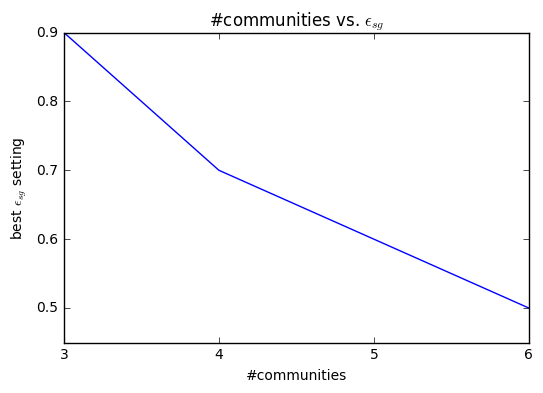
\includegraphics[width=.49\textwidth]{parameter_plot.png}
\caption{Community size against $\epsilon_{sg}$. Communities contained 32 nodes and each node has 16 connections to nodes within its own community, and 16 to nodes outside. NMI scores in bold show the best NMI score for the number of communities. Each setting was repeated 10 times. }
\label{parameter_experiment}
\end{figure}

%\begin{figure}
%\centering
%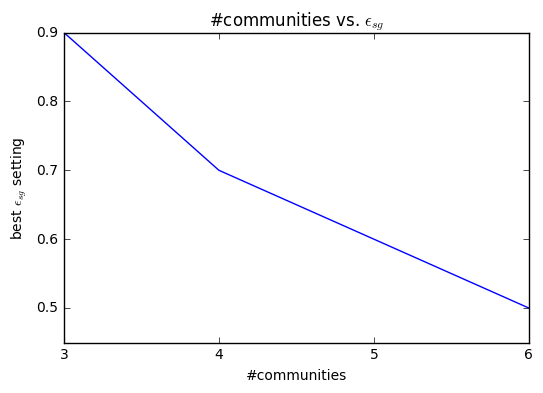
\includegraphics[scale=0.65]{parameter_plot.png}
%\caption{Plot of community size against $\epsilon_{sg}$.}
%\label{parameter_experiment}
%\end{figure}

%TODO talk about density vs e_sg

\begin{figure}
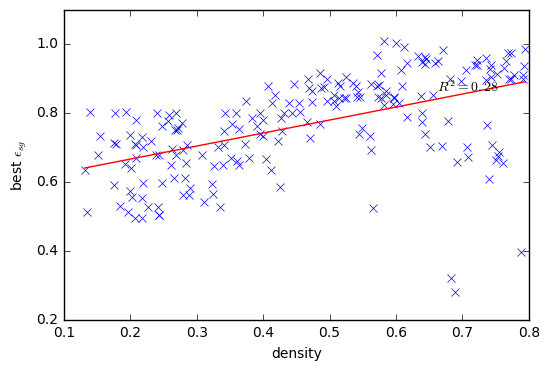
\includegraphics[scale=0.65]{derived_results.png}
\caption{Plot of network density vs. best setting for $\epsilon_{sg}$. 200 random networks of 64 nodes were generated with a random number of edges and communities.}
\end{figure}

\subsection{Synthetic Hierarchical Benchmarks}
In ordert to investigate the strength of GHSOM at uncovering the hierarchical community structure of complex networks, synthetic benchmark networks were generated using software provided by Lancichinetti et al. \cite{lancichinetti2009detecting}. 
The generated networks were comprised of 512 nodes divided into 16 communities of 32 nodes. 
These 16 communities formed 4 super-communities of 128 nodes. 
This produced networks of nodes belonging to communities at two levels: one at the micro level and one at the macro level.

The algorithm allows for the adjustment of three mixing parameters: $z_1, z_2,$ and $z_3$, which control the number of connections between nodes of the same micro community, same macro community and other communities in the network respectively. 
As in \cite{lancichinetti2009detecting} and \cite{yang2013hierarchical}, we keep $z_1$ and $z_2$ fixed at 16, and vary $z_3$, the number of connections between nodes of different macro communities, from 16 to 36, and plot NMI score for both levels of community. 
For $z_3 > 32$ then the external degree of nodes (the number of links outside of their micro/macro community) is greater than their internal degree so searching for communities in this case becomes challenging. 
\Cref{synthetic_experiment} shows a plot of the results of this experiment against three other algorithms from the literature. 
%FM \cite{clauset2004finding}, FUC \cite{blondel2008fast} and PMC \cite{yang2013hierarchical}.

\begin{figure}
\centering
%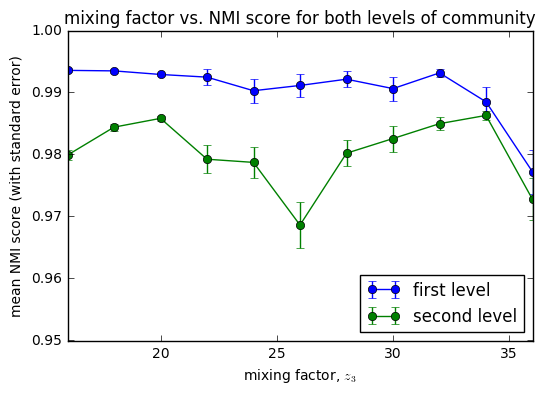
\includegraphics[scale=0.65]{synthetic_results.png}
%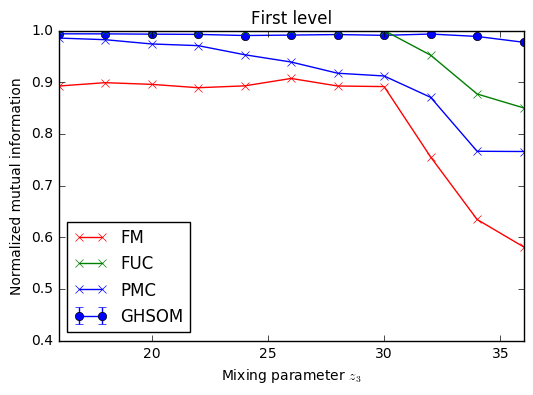
\includegraphics[width=\textwidth]{first_level.png}
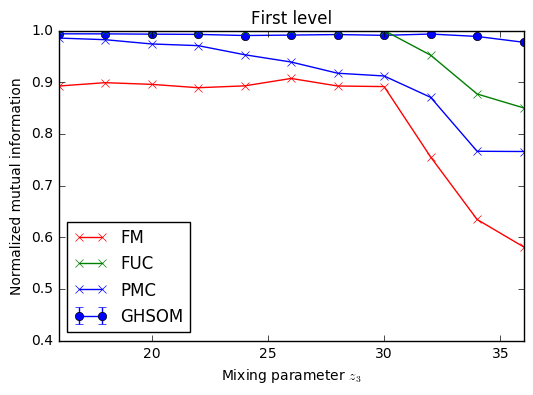
\includegraphics[scale=0.65]{first_level.png}
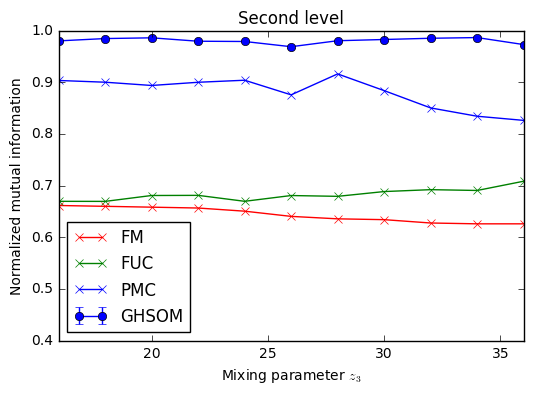
\includegraphics[scale=0.65]{second_level.png}
\caption{Plot of mixing parameter $z_3$ against NMI score for both levels of community. 100 networks were generated with each mixing parameter. Results extracted without permission from \protect\cite{yang2013hierarchical} (fig 4).}
\label{synthetic_experiment}
\end{figure}

%\begin{figure}
%\centering
%%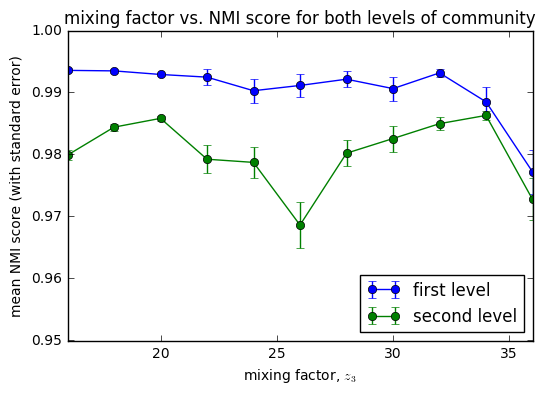
\includegraphics[scale=0.65]{synthetic_results.png}
%%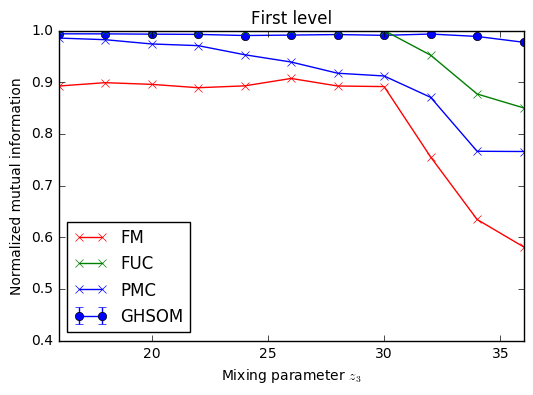
\includegraphics[scale=0.45]{first_level.png}
%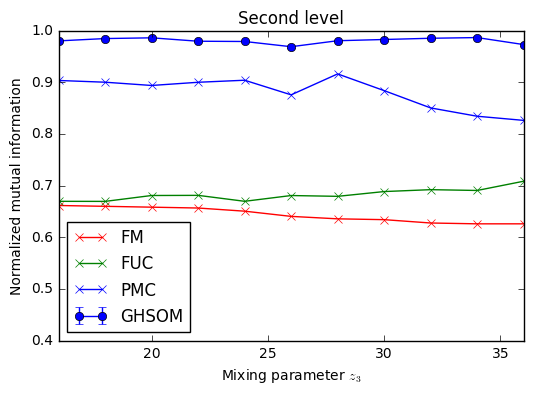
\includegraphics[scale=0.65]{second_level.png}
%\caption{Plot of mixing parameter $z_3$ against NMI score for both levels of community. 100 networks were generated with each mixing parameter. Results extracted without permission from \protect\cite{yang2013hierarchical} (fig 4).}
%\label{synthetic_experiment_2}
%\end{figure}

\subsection{Preserving Topology}

\section{Discussion}
The aim of this study was to investigate the usefulness of GHSOM as a tool for hierarchical community detection. 
We found that GHSOM was capable of community detection on both small real world and synthetic networks. 
With some optimization, GHSOM was able to produce results as good as the other algorithms in the literature on the real world networks (\cref{bayes}). However, the results achieved by the spearmint software are difficult to reproduce and seem to rely heavily on a lucky random initialization.

On the synthetic experiments, GHSOM consistently achieved almost perfect NMI scores for both level of community, even when the external degree of nodes was greater than the internal degree (\cref{synthetic_experiment}).
Both \cite{lancichinetti2009detecting} and \cite{yang2013hierarchical} struggled with these cases and the NMI score for $z_3 > 32$ dropped noticeably (to less than 0.9).
%TODO WHY?
In this author's opinion, this is the result of embedding using MDS. In the cases of $z_3 > 32$, each node had 16 connections to nodes in the same micro community (31 other nodes), 16 connections to nodes in the same macro, but not micro community (96 other nodes) and 32-36 connections to the 384 nodes of the network. 
Even though the external degree of each node was greater than the internal degree, the ratio of connections to possible target nodes was still decreasing.
Because of this, the distance between nodes of different communities was still larger than nodes of the same community and so MDS was able to embed these nodes in such a way that identifying communities was still possible. 
Bonabeau \cite{bonabeau2002graph} cites \cite{kernighan1970efficient} who identified that MDS can allow for clusters and communities within a graph to be more easily identifiable even before a cover is found. 

But, for practical community detection, GHSOM will require some work. 
Firstly, GHSOM showed poor scalability. Self-organizing map algorithms are notorious for issues with scalability \cite{smith2002applications}.
All of the experiments here dealt with small networks (of no more than 512 nodes), but running the algorithm could take upto twenty minutes on a personal laptop.
Clearly, as it is presented in this work, GHSOM cannot scale up to networks of thousands of nodes and still be practical.
Its scalability could be improved, however.
A more intelligent GHSOM implementation would take advantage of GPU processing for the all of the numerical computation.
It should also be noted that the training of separate maps from the same level could be implemented to run in parallel, as they deal with entire separate data points, further speeding up run time.

It was also apparent that, while achieving good NMI scores, the number of neurons in the network could overestimate the number of communities in the network. 
This happened when a neuron was not pointing close to any data points and so was assigned no nodes in the graph.
The error of these neurons was zero and this erroneously brought down the error of the entire map.
This problem was alleviated somewhat by keeping the learning rate small and training for 10000 epochs, rather than the initial 1000, as as to entire the weights moved sufficiently enough to point to the centre of some data points. 
However, a better sampling of the input space when inserting neurons, as well as some form of neuron deletion, would be a fruitful addition in the future.

Only one similarity measure (shortest path distance) was used in this study, however, as previously noted, changing the similarity measure could potentially cause GHSOM to identify different communities. 
An investigation into the impact of the choice of similarity measure and the communities that are conserved across many of them would be an informative future study. 
One such potential metric is the DSD metric of Cao et al., a metric shown to be more suitable for protein-protein interaction (PPI) networks with few nodes of very high degree \cite{cao2013going}. 
One could also experiment with different neuron weight representations, such as the direct-to-graph representation of \cite{yamakawa2006self}, and examine the impact of removing MDS altogether.
Additionally, increasing the dimensinoality of the map representation could potentially remove `false neighbours' from the map \cite{bonabeau2002graph} and present a more accurate representation of the underlying community structure in the data. 
By giving neurons overlapping receptive fields in the input space, one could potentially detect overlapping communities in the network as well as hierachical ones \cite{lancichinetti2009detecting}.

Performance of GHSOM was shown to be heavily dependant upon parameter settings. 
Fine-tuning parameters is a challenging task, but this affords the algorithm a great deal of customizability, especially in the case of exploratory data mining, where community labels are not known a-priori.
One could use the modularity of the communities uncovered as a guide for parameter settings and use a range of parameters to get multiple candidate covers.
Additionally, one could overcome the need for so much difficult fine-tuning of parameters altogether by making the entire algorithm more principled by following the example of Bishop et al. in their Generative Topographical Mapping (GTM) algorithm \cite{bishop1996gtm}.

Overall, GHSOM showed potential as a hierarchical community detection algorithm. 
With some fine-tuning, it achieved good NMI scores on the hierarchical benchmarks, even with the high mixing factor that other algorithms struggled with. 
However, work still needs to be done to deal with issues of scalability and make the entire algorithm more principled. 



%\section*{Acknowledgements}
%
%The author would like to sincerely thank Dr. Shan He for his continual support throughout the work described here in this paper. His knowledge and guidance were integral to the completion of this work, and it would not have been done without him.


%\bibliographystyle{unsrt}
\bibliographystyle{named}
\bibliography{references}

\end{document}

